\documentclass[tikz,border=8pt]{standalone}
\usepackage{amsmath,amssymb}
\usetikzlibrary{arrows.meta,calc,decorations.markings,decorations.pathmorphing,patterns,shapes.geometric,positioning}

\begin{document}
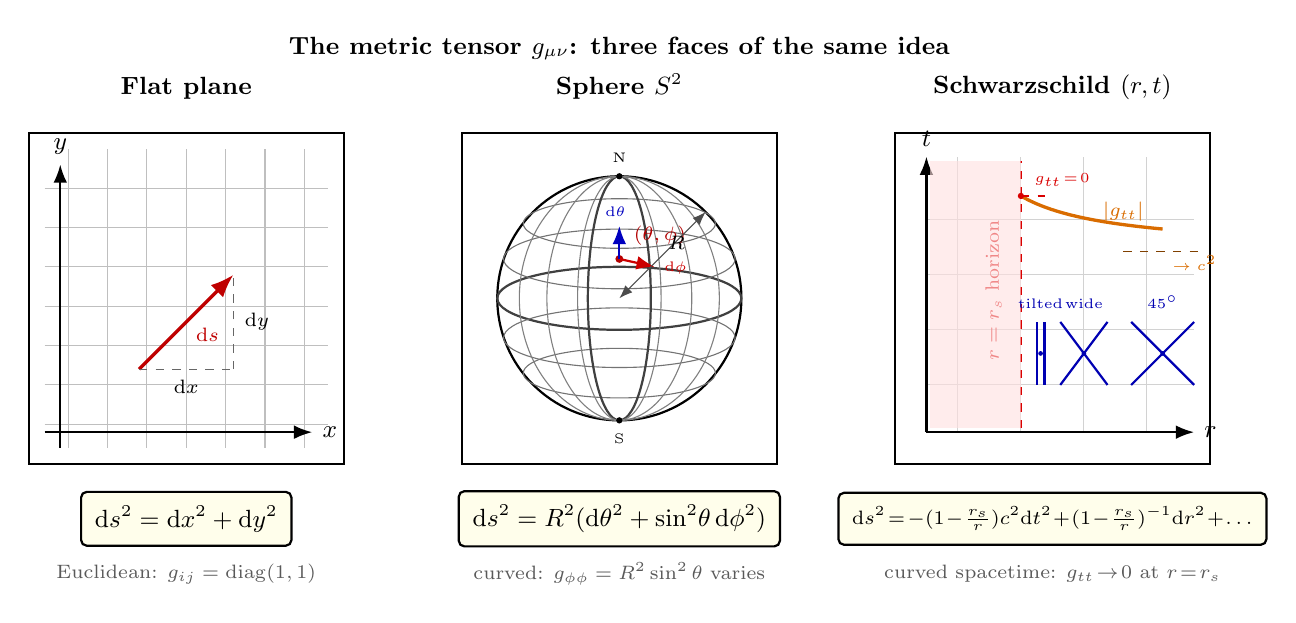
\begin{tikzpicture}[>=Latex]

  % ============================================================
  % LEFT PANEL: Flat plane with grid
  % ============================================================
  \begin{scope}[shift={(0,0)}]
    \node[font=\small\bfseries, anchor=south] at (2.0, 4.5) {Flat plane};

    \draw[black, thick] (0, 0) rectangle (4.0, 4.2);

    % Grid
    \foreach \x in {0.5, 1.0, 1.5, 2.0, 2.5, 3.0, 3.5} {
      \draw[gray!50, thin] (\x, 0.2) -- (\x, 4.0);
    }
    \foreach \y in {0.5, 1.0, 1.5, 2.0, 2.5, 3.0, 3.5} {
      \draw[gray!50, thin] (0.2, \y) -- (3.8, \y);
    }
    % Axes
    \draw[->, thick, black] (0.2, 0.4) -- (3.6, 0.4) node[anchor=west, font=\small]{$x$};
    \draw[->, thick, black] (0.4, 0.2) -- (0.4, 3.8) node[anchor=south, font=\small]{$y$};

    % Sample displacement vector
    \draw[->, very thick, red!75!black] (1.4, 1.2) -- (2.6, 2.4);
    \node[font=\scriptsize, red!75!black, anchor=north west] at (2.0, 1.85) {$\mathrm{d}s$};
    % dx and dy decomposition
    \draw[dashed, black!60] (1.4, 1.2) -- (2.6, 1.2);
    \draw[dashed, black!60] (2.6, 1.2) -- (2.6, 2.4);
    \node[font=\scriptsize, anchor=north] at (2.0, 1.18) {$\mathrm{d}x$};
    \node[font=\scriptsize, anchor=west] at (2.62, 1.8) {$\mathrm{d}y$};

    % Formula box below
    \node[draw=black, thick, fill=yellow!8, rounded corners=2pt,
          font=\small, align=center, inner sep=5pt] at (2.0, -0.7)
      {$\mathrm{d}s^2 = \mathrm{d}x^2 + \mathrm{d}y^2$};
    \node[font=\scriptsize, text=black!65, align=center] at (2.0, -1.4)
      {Euclidean: $g_{ij}=\mathrm{diag}(1,1)$};
  \end{scope}

  % ============================================================
  % MIDDLE PANEL: Sphere with theta-phi grid
  % ============================================================
  \begin{scope}[shift={(5.5,0)}]
    \node[font=\small\bfseries, anchor=south] at (2.0, 4.5) {Sphere $S^2$};

    \draw[black, thick] (0, 0) rectangle (4.0, 4.2);

    % Sphere parameters
    \def\cx{2.0}
    \def\cy{2.1}

    % Outer circle (silhouette) - radius 1.55
    \draw[black, thick] (\cx, \cy) circle [radius=1.55];

    % Equator (ellipse, perspective)
    \draw[black!75, thick] (\cx, \cy) ellipse [x radius=1.55, y radius=0.4];

    % Latitude circles (parallels) - ellipses
    \foreach \dy/\rr/\ey in {0.95/1.22/0.315, 0.5/1.47/0.379, -0.5/1.47/0.379, -0.95/1.22/0.315} {
      \draw[black!55, thin] (\cx, \cy+\dy) ellipse [x radius=\rr, y radius=\ey];
    }

    % Front meridian (vertical major axis)
    \draw[black!75, thick] (\cx, \cy) ellipse [x radius=0.4, y radius=1.55];

    % Tilted meridians (different x-radii)
    \foreach \xr in {1.27, 0.92, 0.53} {
      \draw[black!50, thin] (\cx, \cy) ellipse [x radius=\xr, y radius=1.55];
    }

    % Highlight a "small piece" near a non-equator latitude
    \def\px{2.0}
    \def\py{2.6}
    \fill[red!70!black] (\px, \py) circle [radius=0.05];
    \node[font=\scriptsize, red!70!black, anchor=south west] at (\px+0.06, \py+0.05) {$(\theta,\phi)$};

    % theta and phi arrows
    \draw[->, thick, red!80!black] (\px, \py) -- (\px+0.45, \py-0.10);
    \draw[->, thick, blue!75!black] (\px, \py) -- (\px+0.0, \py+0.42);
    \node[font=\tiny, red!80!black, anchor=west] at (\px+0.45, \py-0.12) {$\mathrm{d}\phi$};
    \node[font=\tiny, blue!75!black, anchor=south] at (\px-0.05, \py+0.42) {$\mathrm{d}\theta$};

    % Pole markers
    \fill[black] (\cx, \cy+1.55) circle [radius=0.04];
    \fill[black] (\cx, \cy-1.55) circle [radius=0.04];
    \node[font=\tiny, anchor=south] at (\cx, \cy+1.55+0.05) {N};
    \node[font=\tiny, anchor=north] at (\cx, \cy-1.55-0.05) {S};

    % R label
    \draw[<->, thin, black!70] (\cx, \cy) -- ($(\cx,\cy)+(45:1.55)$);
    \node[font=\scriptsize, anchor=south west] at ($(\cx,\cy)+(45:0.7)$) {$R$};

    % Formula box below
    \node[draw=black, thick, fill=yellow!8, rounded corners=2pt,
          font=\small, align=center, inner sep=5pt] at (2.0, -0.7)
      {$\mathrm{d}s^2 = R^2(\mathrm{d}\theta^2 + \sin^2\!\theta\,\mathrm{d}\phi^2)$};
    \node[font=\scriptsize, text=black!65, align=center] at (2.0, -1.4)
      {curved: $g_{\phi\phi}=R^2\sin^2\theta$ varies};
  \end{scope}

  % ============================================================
  % RIGHT PANEL: Schwarzschild (r-t plane)
  % ============================================================
  \begin{scope}[shift={(11.0,0)}]
    \node[font=\small\bfseries, anchor=south] at (2.0, 4.5) {Schwarzschild $(r,t)$};

    \draw[black, thick] (0, 0) rectangle (4.0, 4.2);

    \def\rs{1.2}
    \def\xleft{0.4}
    \def\xright{3.8}
    \def\ybot{0.4}
    \def\ytop{3.9}

    % Grid (faint)
    \foreach \x in {0.8, 1.6, 2.4, 3.2} {
      \draw[gray!35, thin] (\x, \ybot) -- (\x, \ytop);
    }
    \foreach \y in {1.0, 1.7, 2.4, 3.1} {
      \draw[gray!35, thin] (\xleft, \y) -- (\xright, \y);
    }

    % Axes
    \draw[->, thick, black] (\xleft, \ybot) -- (\xright, \ybot) node[anchor=west, font=\small]{$r$};
    \draw[->, thick, black] (\xleft, \ybot) -- (\xleft, \ytop) node[anchor=south, font=\small]{$t$};

    % Horizon line: r = r_s (red dashed vertical)
    \draw[red!85!black, thick, dashed] (\xleft+\rs, \ybot+0.05) -- (\xleft+\rs, \ytop-0.05);
    \node[font=\scriptsize, red!85!black, anchor=south, rotate=90] at (\xleft+\rs-0.12, 2.2) {$r=r_s$ horizon};

    % Shaded forbidden region (r < r_s)
    \fill[red!12, opacity=0.6] (\xleft+0.05, \ybot+0.05) rectangle (\xleft+\rs, \ytop-0.05);

    % Light-cone sketches
    % near r_s: very tilted (almost vertical)
    \begin{scope}[shift={(\xleft+\rs+0.25, 1.4)}]
      \draw[blue!70!black, thick] (-0.05, -0.4) -- (-0.05, 0.4);
      \draw[blue!70!black, thick] (0.05, -0.4) -- (0.05, 0.4);
      \fill[blue!70!black] (0, 0) circle [radius=0.03];
    \end{scope}
    \node[font=\tiny, blue!70!black, anchor=south] at (\xleft+\rs+0.25, 1.85) {tilted};

    % medium r
    \begin{scope}[shift={(\xleft+2.0, 1.4)}]
      \draw[blue!70!black, thick] (-0.30, -0.4) -- (0.30, 0.4);
      \draw[blue!70!black, thick] (0.30, -0.4) -- (-0.30, 0.4);
      \fill[blue!70!black] (0, 0) circle [radius=0.03];
    \end{scope}
    \node[font=\tiny, blue!70!black, anchor=south] at (\xleft+2.0, 1.85) {wide};

    % far r: 45 deg, Minkowski-like
    \begin{scope}[shift={(\xleft+3.0, 1.4)}]
      \draw[blue!70!black, thick] (-0.40, -0.4) -- (0.40, 0.4);
      \draw[blue!70!black, thick] (0.40, -0.4) -- (-0.40, 0.4);
      \fill[blue!70!black] (0, 0) circle [radius=0.03];
    \end{scope}
    \node[font=\tiny, blue!70!black, anchor=south] at (\xleft+3.0, 1.85) {$45^\circ$};

    % |g_tt| qualitative curve
    \draw[orange!85!black, very thick, smooth, samples=40, domain=1.21:3.0]
      plot ({\xleft+\x}, {3.4 - 0.7*(1 - 1.2/\x)});
    \node[font=\scriptsize, orange!85!black, anchor=south] at (\xleft+2.5, 2.95) {$|g_{tt}|$};

    % g_tt = 0 mark
    \draw[red!85!black, dashed, thin] (\xleft+\rs, 3.4) -- (\xleft+\rs+0.3, 3.4);
    \fill[red!85!black] (\xleft+\rs, 3.4) circle [radius=0.04];
    \node[font=\tiny, red!85!black, anchor=west] at (\xleft+\rs+0.05, 3.6) {$g_{tt}\!=\!0$};

    % Asymptote to -c^2 at large r
    \draw[orange!50!black, dashed, thin] (\xleft+2.5, 2.7) -- (\xleft+3.5, 2.7);
    \node[font=\tiny, orange!85!black, anchor=west] at (\xleft+3.0, 2.55) {$\to c^2$};

    % Formula box
    \node[draw=black, thick, fill=yellow!8, rounded corners=2pt,
          font=\scriptsize, align=center, inner sep=5pt] at (2.0, -0.7)
      {$\mathrm{d}s^2 \!=\! -(1\!-\!\tfrac{r_s}{r})c^2\mathrm{d}t^2 \!+\! (1\!-\!\tfrac{r_s}{r})^{-1}\mathrm{d}r^2 \!+\! \ldots$};
    \node[font=\scriptsize, text=black!65, align=center] at (2.0, -1.4)
      {curved spacetime: $g_{tt}\!\to\!0$ at $r\!=\!r_s$};
  \end{scope}

  % ============================================================
  % Top caption
  % ============================================================
  \node[font=\small\bfseries, anchor=south] at (7.5, 5.0)
    {The metric tensor $g_{\mu\nu}$: three faces of the same idea};

\end{tikzpicture}
\end{document}
